\documentclass{article}

\usepackage{amsmath, amsthm, amssymb, amsfonts}
\usepackage{tikz-cd}
\usepackage{thmtools}
\usepackage{graphicx}
\usepackage{setspace}
\usepackage{geometry}
\usepackage{float}
\usepackage{hyperref}
\usepackage[utf8]{inputenc}
\usepackage[english]{babel}
\usepackage{framed}
\usepackage[dvipsnames]{xcolor}
\usepackage{tcolorbox}
\usepackage{tikz}
\usetikzlibrary{patterns}
\colorlet{LightGray}{White!90!Periwinkle}
\colorlet{LightOrange}{Orange!15}
\colorlet{LightGreen}{Green!15}

\newcommand{\HRule}[1]{\rule{\linewidth}{#1}}

\declaretheoremstyle[name=,]{thmsty}
\declaretheorem[style=thmsty,numberwithin=section]{theorem}
\tcolorboxenvironment{theorem}{colback=LightGray}

\declaretheoremstyle[name=,]{prosty}
\declaretheorem[style=prosty,numberlike=theorem]{notes}
\tcolorboxenvironment{proposition}{colback=LightOrange}

\declaretheoremstyle[name=,]{prcpsty}
\declaretheorem[style=prcpsty,numberlike=theorem]{question}
\tcolorboxenvironment{principle}{colback=LightGreen}

\setstretch{1.2}
\geometry{
    textheight=9in,
    textwidth=5.5in,
    top=1in,
    headheight=12pt,
    headsep=25pt,
    footskip=30pt
}

% ------------------------------------------------------------------------------

\begin{document}

% ------------------------------------------------------------------------------
% Cover Page and ToC
% ------------------------------------------------------------------------------

\title{ \normalsize \textsc{Lie Groups and Lie Algebra}
		\\ [2.0cm]
		\HRule{1.5pt} \\
        \LARGE \textbf{\uppercase{A lecture note on SuperConductivity for Noob Wannabe Physicists}
		\HRule{2.0pt} \\ [0.6cm] \LARGE{} \vspace*{10\baselineskip}}
		}
        %\date{}
\author{\textbf{Author} \\ 
		Mushrafi Munim Sushmit \\
		Department of Physics, University of Dhaka \\
		}

\maketitle
\newpage

\tableofcontents
\newpage

\section*{Preface} % The asterisk prevents LaTeX from numbering the section
\addcontentsline{toc}{section}{Preface} 

This document draws primarily from the online lectures delivered by Dr. Ratan Chandra Ghosh, which are available on YouTube.
\newpage 

\subsection{Introduction}

In 1957, Bardeen, Cooper, and Schrieffer (BCS) introduced a groundbreaking theory of superconductivity, commonly known as the BCS theory. This theory demonstrated that even a weak attractive interaction between electrons, mediated by second-order electron-phonon interactions, could destabilize the conventional Fermi-sea ground state of an electron gas. This instability leads to the formation of bound pairs of electrons, known as \textit{Cooper pairs}, where the electrons occupy states with equal and opposite momentum and spin. These Cooper pairs possess a spatial extension of the order of $\xi_0$ and represent the superconducting charge carriers predicted by earlier phenomenological models.

A central prediction of the BCS theory is the requirement of a minimum energy,

\[
E_k = 2\Delta(T),
\]

to break a Cooper pair, resulting in the creation of two quasi-particle excitations. The energy gap $\Delta(T)$ increases from zero at the critical temperature $T_c$ to a limiting value at low temperatures,

\[
E_k(0) = 2\Delta(0) = 3.528 k T_c \tag{1}
\]

for $T \ll T_c$. This prediction closely matched experimental measurements of the gap width, and the BCS model for the absorption edge, above the energy threshold $\hbar \omega_g = E_g$, was in strong agreement with experimental data from Glover and Tinkham. This consistency between theory and experiment provided one of the earliest and most definitive confirmations of the BCS microscopic theory of superconductivity.

\subsection{Electron Pairing and BCS Theory}

Consider a metal in which the conduction electrons lie inside the Fermi sphere. Suppose that two electrons lie just inside the Fermi surface, as shown in the following figure, and repel each other because of Coulomb interaction.

\begin{center}
    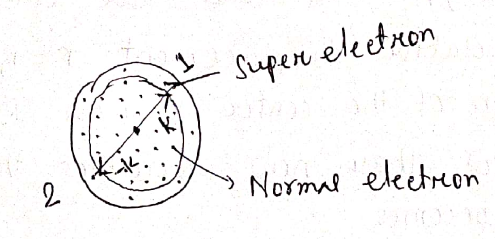
\includegraphics[width=0.4\textwidth]{figures/fermi_sphere.png} \\
    Figure: Super electron and normal electron inside the Fermi sphere
\end{center}

But this Coulomb force is reduced substantially on account of the screening due to the presence of other electrons in the Fermi sphere. After the screening is taken into account, the interaction between the two electrons disappears almost entirely.

Suppose that, for some reason, the two electrons attract each other, something new may occur. Cooper showed that the two electrons would form a bound state, electrons in which are paired to form a single system and their motions are correlated.

Consider two electrons that interact with each other via an attractive potential $U(r_1 - r_2)$. The Schrödinger equation is given by:

\[
\left[ -\frac{\hbar^2 \nabla_{r_1}^2}{2m} - \frac{\hbar^2 \nabla_{r_2}^2}{2m} + V(r_1 - r_2) \right] \psi(r_1, r_2) = E \psi(r_1, r_2) \tag{1}
\]

Where $\psi(r_1, r_2)$ is the wavefunction and $E$ is the energy. As usual, we change variables to the relative displacement $r = r_1 - r_2$ and to the position of the center of mass $R = \frac{1}{2}(r_1 + r_2)$. In terms of these new variables, the Schrödinger equation becomes:

\[
\left[ -\frac{\hbar^2 \nabla_{R}^2}{2m^*} - \frac{\hbar^2 \nabla_{r}^2}{2\mu} + V(r) \right] \psi(r, R) = E \psi(r, R) \tag{2}
\]

Where $m^* = 2m$ is the total mass and $\mu = m/2$ is the reduced mass. Since the potential does not depend on the center of mass coordinate $R$, we look for a solution:

\[
\psi(r, R) = \psi(r) e^{-i\mathbf{k} \cdot \mathbf{R}} \tag{3}
\]

After substitution of equation (3) into equation (2), we get:

\[
\left[ -\frac{\hbar^2 \nabla_{r}^2}{2\mu} + V(r) \right] \psi(r) = E' \psi(r) \tag{4}
\]

Where $E' = E - \frac{\hbar^2 k^2}{2m^*}$. For a given $E$ eigenvalue, the lowest energy $E$ is the one for which $\mathbf{k} = 0$, that is, for which the momentum of the center of mass vanishes.

\subsection{Formation of Cooper Pairs}

We have been discussing the consequences of electron-electron attraction, but how does this attraction come about in the first place? In superconductive materials, it results from the electron-lattice interaction, as shown in Fig. 10.16.

\begin{center}
    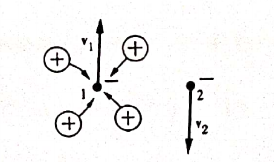
\includegraphics[width=0.4\textwidth]{figures/electron_lattice_interaction.png} \\
    Figure 10.16: The screening of electron 1 by the positive ions of the lattice. Solid circles represent the two electrons considered.
\end{center}

Suppose that the two electrons, 1 and 2, pass each other. Because electron 1 is negatively charged, it attracts positive ions toward itself (electron-lattice interaction). Thus, electron 2 does not “see” the bare electron 1. Electron 1 is screened by ions. The screening may greatly reduce the effective charge of this electron; in fact, the ions may overrespond and produce a net positive charge. If this happens, then electron 2 will be attracted toward it. This leads to a net attractive interaction, as required for the formation of the Cooper pair.

The ions' overresponse may be understood qualitatively. Since electron 1 is near the Fermi surface, its speed is great. At the same time, the ions, because of their heavy masses, respond rather slowly. By the time they have felt and completely responded to electron 1, electron 1 has left its initial region, at least partially, thus stimulating the overcompensation. One can also reason that this process is most effective when electron 1 and electron 2 move in opposite directions.

In technical literature, one says that each electron is surrounded by a “phonon cloud,” and that the two electrons establish an attractive interaction by exchanging phonons; for example, electron 1 emits phonons which are very quickly absorbed by electron 2. Since the phonon is involved twice—once in emission and once in absorption—the attraction between electrons is a second-order process.

As a result of this binding between electron 1 and electron 2, an energy gap appears in the spectrum of the electron. This gap straddles the Fermi energy level.

\subsection{Scattering of Cooper Pairs}

Let us consider two electrons above a filled Fermi sphere. These two electrons are attracted by the exchange of phonons. However, the maximum energy which may be exchanged by this way is $\sim \hbar \omega_D$. Thus the scattering in phase space is restricted to a narrow shell of energy width $\hbar \omega_D$. Furthermore, the momentum in this scattering process is also conserved.

\[
\mathbf{k_1} + \mathbf{k_2} = \mathbf{k_1'} + \mathbf{k_2'} = \mathbf{K}
\]

\begin{center}
    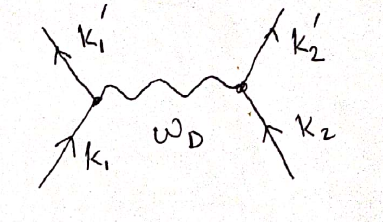
\includegraphics[width=0.3\textwidth]{figures/scattering_diagram_1.png}
\end{center}

Thus the scattering of $\mathbf{k_1}$ and $\mathbf{k_2}$ into $\mathbf{k_1'}$ and $\mathbf{k_2'}$ is restricted to the overlap of the two scattering shells, meaning this is negligible unless $\mathbf{K} \approx 0$. Thus, the interaction is strongest if $\mathbf{k_1} = -\mathbf{k_2}$ and $\sigma_1 = -\sigma_2$; pairing is primarily between time-reversed eigenstates.

\begin{center}
    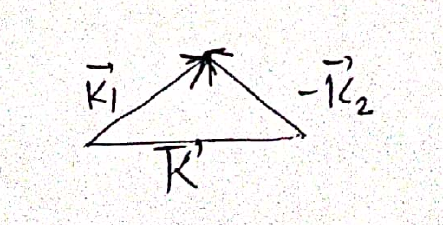
\includegraphics[width=0.3\textwidth]{figures/scattering_diagram_2.png}
\end{center}

The net effect of the phonons is then to create an attractive interaction which tends to pair time-reversed quasiparticle states. They form an antisymmetric spin singlet so that the spatial part of the wavefunction can be symmetric and nodeless and so take advantage of the attractive interaction.

\begin{center}
    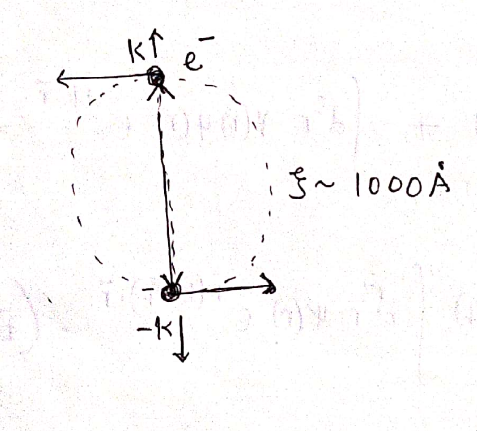
\includegraphics[width=0.3\textwidth]{figures/pairing.png} \\
    Figure: Cooper pair formation
\end{center}

Depending on the symmetry of the spatial part of the wavefunction, even $\psi(r) = \psi(-r)$ or odd $\psi(r) = -\psi(-r)$, the spins of the electrons will form either a singlet or a triplet state, respectively, in order to ensure the anti-symmetry of the total wavefunction.

We know from the definition of the Fourier transformation:
\[
\psi(\mathbf{k}) = \int d^3r \, \psi(\mathbf{r}) e^{-i\mathbf{k} \cdot \mathbf{r}} \tag{1}
\]

We know
\[
\left[ -\frac{\hbar^2 \nabla_r^2}{2\mu} + V(r) \right] \psi(r) = E \psi(r) \tag{*1}
\]
Using the definition of the Fourier transformation in equation (*1) gives
\[
\frac{\hbar^2 k^2}{2\mu} \psi(\mathbf{k}) + \int d^3r \, V(r) \psi(r) e^{-i\mathbf{k} \cdot \mathbf{r}} = E \psi(\mathbf{k}) \tag{*2}
\]
Now defining new variables $\mathbf{q} = \mathbf{k} - \mathbf{k}'$ (free electron energy $\epsilon_k = \frac{\hbar^2 k^2}{2m}$), equation (*2) gives
\[
\int \frac{d^3 k'}{(2\pi)^3} V(\mathbf{k} - \mathbf{k'}) \psi(\mathbf{k'}) = (E - 2\epsilon_k) \psi(\mathbf{k}) \tag{*3}
\]

A bound state between two electrons has $E < 2\epsilon_k$, i.e., the total energy is smaller than the energy of two independent free electrons. Therefore, we define the modified wavefunction as
\[
\Delta(\mathbf{k}) = (E - 2\epsilon_k) \psi(\mathbf{k}) \tag{*4}
\]
Using this we can write equation (*3) as
\[
\Delta(\mathbf{k}) = - \int \frac{d^3 k'}{(2\pi)^3} \frac{V(\mathbf{k} - \mathbf{k'})}{2\epsilon_{k'} - E} \Delta(\mathbf{k'}) \tag{*5}
\]
Equation (*5) is just the Schrödinger equation written in a different form.

Now let us consider a potential that is attractive, $V(\mathbf{k} - \mathbf{k'}) = -V_0$, for $\epsilon_k, \epsilon_{k'} < \hbar \omega_D$ and zero otherwise. Now we look for a solution of equation (*5).

According to Fermi-Dirac statistics, the density of states per spin is
\[
\rho(E) = \frac{m^{3/2}}{\sqrt{2} \hbar^3 \pi^2} \sqrt{E} \tag{*6}
\]

We obtain
\[
\Delta = \frac{V_0 \Delta m^{3/2}}{\sqrt{2} \hbar^3 \pi^2} \int_0^{\hbar \omega_D} \frac{\sqrt{\epsilon} d\epsilon}{2\epsilon - E} \tag{*7}
\]
or
\[
1 = \frac{V_0 m^{3/2}}{\sqrt{2} \hbar^3 \pi^2} \left[ \sqrt{\hbar \omega_D} - \sqrt{\frac{-E}{2}} \tan^{-1}\left( \sqrt{\frac{2\hbar \omega_D}{-E}} \right) \right]
\]
This equation determines the value of the bound state energy $E < 0$ as a function of the attractive potential $V_0$. In order to have a bound state, we set $E \to 0^-$ to obtain the minimum value of $V_0$
\[
V_{0, \text{min}} = \frac{\sqrt{2} \hbar^3 \pi^2}{m^{3/2} \sqrt{\hbar \omega_D}} \tag{*8}
\]
Equation (*8) tells us that there will be a bound state only if the attractive interaction is strong enough.

Now we consider the potential \( V(\vec{k} - \vec{k'}) = -V_0 \) for the unoccupied electronic states above the Fermi energy \( E_F \), \( \epsilon_{k'} - E_F \), \( \epsilon_k - E_F < \hbar \omega_D \).

Since \( \hbar \omega_D \ll E_F \), we can approximate the density of states for its value at \( E_F \).

Now equation (5) becomes, for \( \Delta(k) = \Delta \):

\[
\Delta = V_0 P(E_F) \Delta \int_{E_F}^{E_F + \omega_D} \frac{d\epsilon}{2\epsilon - E}
\]

\[
1 = V_0 P(E_F) \cdot \frac{1}{2} \left| \ln(2\epsilon - E) \right|_{E_F}^{E_F + \omega_D}
\]

\[
\frac{2}{V_0 P(E_F)} = \ln \left( \frac{2E_F + 2\omega_D - E}{2E_F - E} \right) = \ln \left( 1 + \frac{2\omega_D}{2E_F - E} \right)
\]

In the limit where \( V_0 P(E_F) \ll 1 \) and \( E \) is close to \( 2E_F \), we approximate \( 2E_F - E + 2\omega_D \approx 2\omega_D \).

Defining the binding energy \( E_b = 2E_F - E \), we obtain:

\[
\frac{2}{V_0 P(E_F)} = \ln \left( \frac{E_b + 2\omega_D}{E_b} \right) = \ln \left( 1 + \frac{2\omega_D}{E_b} \right)
\]

\[
\frac{2\omega_D}{E_b} = e^{\frac{2}{V_0 P(E_F)}}
\]

Thus, the binding energy is:

\[
E_b = 2\omega_D e^{-\frac{2}{V_0 P(E_F)}}
\]

This shows that a bound state will be formed regardless of how small the attractive interaction \( V_0 \) is. Such a bound state is called a Cooper pair.

The total energy in the case when there is a center of mass (CM) with a finite momentum \( \vec{K} \) is given below:

\[
E = E_{K=0} + \frac{\hbar^2 K^2}{4m}
\]

\[
E = 2E_F - E_b + \frac{\hbar^2 K^2}{4m}
\]

Here, \( m^* = 2m \).

In the limit \( E \to 2E_F \), we obtain a bound state with a finite CM momentum:

\[
K = \sqrt{\frac{4m E_b}{\hbar^2}} = \frac{2}{\hbar} \sqrt{m E_b}
\]

This finite CM momentum gives rise to a finite current density:

\[
J = n_s e \frac{\hbar K}{m} = 2n_s e \sqrt{\frac{E_b}{m}}
\]

\subsection{BCS Ground State}

In the last section, we have seen that the weak phonon-mediated attractive interaction was sufficient to destabilize the Fermi sea and promote the formation of a Cooper pair \( (k \uparrow, -k \downarrow) \). The scattering from \( (k \uparrow, -k \downarrow) \) to \( (k' \downarrow, -k' \uparrow) \) yields an energy \( V_0 \) to \( k \) and \( k' \), and the scattering shell \( E_F < \epsilon_k, \epsilon_{k'} < E_F + \hbar \omega_D \).

Many electrons can participate in this process, and many Cooper pairs are formed, yielding a new state (phase) of the system. The energy of this new state is not just \( \frac{N}{2} \epsilon \) less than that of the old state, since the Fermi surface is renormalized by the formation of each Cooper pair.

\subsubsection{The Energy of the BCS Ground State}

To study the thermodynamics of this new phase, it is necessary to determine its energy. It will have both kinetic and potential contributions.

Since the pairing of electrons occurs above the Fermi surface, the kinetic energy actually increases. \( \omega_k \) is the probability that a pair state \( (k \uparrow, -k \downarrow) \) is occupied.

\[
E_{\text{Kin}} = 2 \sum_k \omega_k \epsilon_k
\]

\[
\epsilon_k = \frac{\hbar^2 k^2}{2m} - E_F \tag{1}
\]

Potential energy can be written in terms of annihilation and creation operators for paired states labeled by \( k \):

\[
|1\rangle_k \quad (k \uparrow, -k \downarrow) \quad \text{occupied}
\]

\[
|0\rangle_k \quad (k \uparrow, -k \downarrow) \quad \text{unoccupied}
\]

Or,

\[
|\psi_k\rangle = u_k |0\rangle_k + v_k |1\rangle_k \tag{2}
\]

Where \( v_k^2 + u_k^2 = 1 \) is the normalization condition.

Here, \( u_k^2 = \omega_k \) and \( v_k^2 = 1 - \omega_k \).

Therefore, the BCS ground state, which is a collection of these pairs, may be written as:

\[
|\Phi_{\text{BCS}}\rangle \simeq \prod_k \left( u_k |0\rangle_k + v_k |1\rangle_k \right) \tag{3}
\]

We will assume that \( u_k, v_k \in \mathbb{R} \).

Now, according to the Pauli principle, the state \( (k \uparrow, -k \downarrow) \) can be, at most, singly occupied. That is, for \( s = \frac{1}{2} \), the Pauli possible representation is:

\[
|1\rangle_k = \begin{pmatrix} 1 \\ 0 \end{pmatrix}_k, \quad |0\rangle_k = \begin{pmatrix} 0 \\ 1 \end{pmatrix}_k
\]

If \( \sigma_k^+ \) and \( \sigma_k^- \) describe the creation and annihilation operators of the state \( (k \uparrow, -k \downarrow) \), we have:

\[
\sigma_k^+ = \frac{1}{2} \left( \sigma_k^1 + i \sigma_k^2 \right) = \begin{pmatrix} 0 & 1 \\ 0 & 0 \end{pmatrix}
\]

\[
\sigma_k^- = \frac{1}{2} \left( \sigma_k^1 - i \sigma_k^2 \right) = \begin{pmatrix} 0 & 0 \\ 1 & 0 \end{pmatrix}
\]

\[
\sigma_k^+ \begin{pmatrix} 0 \\ 1 \end{pmatrix} = \begin{pmatrix} 1 \\ 0 \end{pmatrix}
\]

\[
\sigma_k^+ |1\rangle_k = 0, \quad \sigma_k^+ |0\rangle_k = |1\rangle_k
\]

\[
\sigma_k^- |1\rangle_k = |0\rangle_k, \quad \sigma_k^- |0\rangle_k = 0
\]

The process \( (k \uparrow, -k \downarrow) \rightarrow (k' \uparrow, -k' \downarrow) \), if allowed, is associated with an energy reduction \( V_0 \). In our Pauli matrix representation, this process is represented by operators \( \sigma_k^+ \sigma_{k'}^- \), so:

\[
V = - \frac{V_0}{(2\pi)^3} \sum_{k k'} \sigma_k^+ \sigma_{k'}^-
\]

Thus, the reduction of the potential energy is given by \( \langle \Phi_{\text{BCS}} | V | \Phi_{\text{BCS}} \rangle \):

\[
\langle \Phi_{\text{BCS}} | V | \Phi_{\text{BCS}} \rangle = - \frac{V_0}{(2\pi)^3} \left\{ \prod_p \left( u_p \langle 0 | + v_p \langle 1 | \right) \sum_{k k'} \sigma_k^+ \sigma_{k'}^- \prod_p \left( u_p |0\rangle_p + v_p |1\rangle_p \right) \right\}
\]

\textbf{Applying the condition:}

\[
\langle 1 1 |_{k k'} = \delta_{k k'}, \quad \langle 0 1 0 |_{k k'} = \delta_{k k'}, \quad \langle 0 1 1 |_{k k'} = 0
\]

\[
\langle \Phi_{\text{BCS}} | V | \Phi_{\text{BCS}} \rangle = -\frac{V_0}{(2\pi)^3} \sum_{k k'} u_k u_k' v_k v_k'
\]

Thus, the total energy (kinetic energy plus potential) of the system of Cooper pairs is:

\[
W_{\text{BCS}} = 2 \sum_k \omega_k^2 \epsilon_k - \frac{V_0}{(2\pi)^3} \sum_{k k'} u_k u_k' v_k v_k'
\]

Now we want to determine \( u_k \) and \( v_k \) appearing in equation (1). Since \( \omega_k = v_k^2 \) and \( 1 - \omega_k = u_k^2 \), we may impose the constraint by choosing:

\[
u_k = \cos \theta_k \quad \text{and} \quad v_k = \sin \theta_k \tag{5}
\]

At \( T = 0 \), we require \( W_{\text{BCS}} \) to be a minimum:

\[
W_{\text{BCS}} = \sum_k 2 \epsilon_k \cos^2 \theta_k - \frac{V_0}{(2\pi)^3} \sum_{k k'} \cos \theta_k \sin \theta_k' \cos \theta_k' \sin \theta_k
\]

\[
= \sum_k 2 \epsilon_k \cos^2 \theta_k - \frac{V_0}{(2\pi)^3} \sum_{k k'} \frac{1}{4} \sin 2\theta_k \sin 2\theta_k' \tag{6}
\]

\[
\frac{\partial W_{\text{BCS}}}{\partial \theta_k} = 0
\]

\[
-4 \epsilon_k \cos \theta_k \sin \theta_k - \frac{V_0}{(2\pi)^3} \sum_{k'} \cos 2\theta_{k'} \sin 2\theta_k = 0
\]

or

\[
\epsilon_k \tan 2\theta_k = -\frac{1}{2} \frac{V_0}{(2\pi)^3} \sum_{k'} \sin 2\theta_{k'}
\]

Conveniently, we can introduce a parameter \( E_k \):

\[
E_k = \sqrt{\epsilon_k^2 + \Delta^2}
\]

where

\[
\Delta = \frac{V_0}{(2\pi)^3} \sum_k u_k v_k
\]

or equivalently

\[
\epsilon_k \tan 2\theta_k = -\frac{\Delta}{E_k} \tag{*1}
\]

Now, using \( 2 u_k v_k = \sin 2\theta_k = \frac{\Delta}{E_k} \) and \( \cos 2\theta_k = \frac{-\epsilon_k}{E_k} \), we obtain:

\[
\cos^2 \theta_k = u_k^2 = \frac{1}{2} \left( 1 + \frac{-\epsilon_k}{E_k} \right)
\]

\[
\omega_k = v_k^2 = \frac{1}{2} \left( 1 - \frac{\epsilon_k}{E_k} \right)
\]

This gives:

\[
\omega_k = v_k^2 = \frac{1}{2} \left( 1 - \frac{\epsilon_k}{\sqrt{\epsilon_k^2 + \Delta^2}} \right)
\]

(Refer to equation 4)

Below is a graph plotting \( \omega_k = v_k^2 \) versus \( \epsilon_k \) at \( T = 0 \):

\begin{figure}[!htbp]
        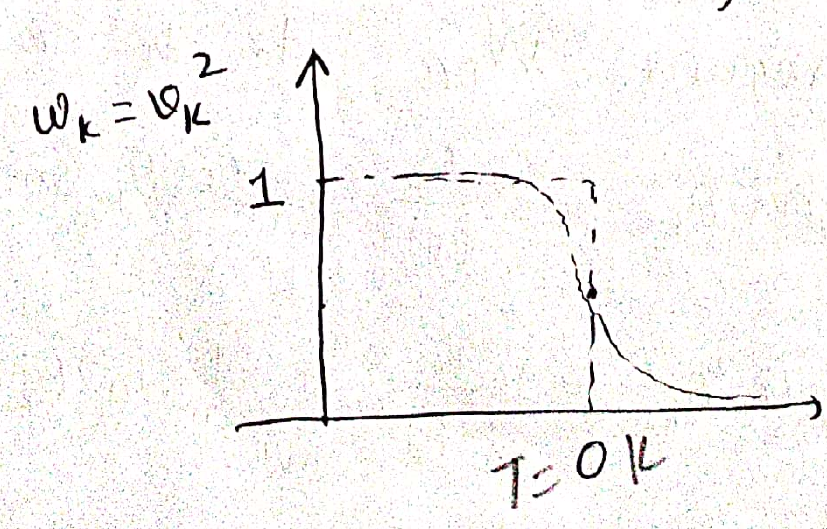
\includegraphics[width=0.35\textwidth]{figures/epsilon_k.png}
    \caption{Graph plotting \( \omega_k \) vs \( \epsilon_k \) showing behavior at \( T = 0 \) }\label{fig:}
\end{figure}

Here,

\[
\epsilon_k = -E_F + \frac{\hbar^2 k^2}{2m}
\]

Now, if we make substitutions \( 2u_k v_k = \frac{\Delta}{E_k} \) and \( v_k^2 = \frac{1}{2} \left( 1 - \frac{\epsilon_k}{E_k} \right) \) into \( W_{\text{BCS}} \), we get:

\[
W_{\text{BCS}} = \sum_k \epsilon_k \left( 1 - \frac{\epsilon_k}{E_k} \right) - \frac{(2\pi)^3}{V_0} \Delta^2
\]

Compare this to the normal state energy, again measured relative to \( E_F \):

\[
W_n = \sum_{k < k_F} 2\epsilon_k
\]

or

\[
\frac{W_{\text{BCS}} - W_n}{(2\pi)^3} = - \frac{1}{(2\pi)^3} \sum_k \epsilon_k \left( 1 + \frac{\epsilon_k}{E_k} \right) - \frac{\Delta^2}{V_0}
\]

\[
\approx - \frac{1}{2} P(E_F) \Delta^2 < 0
\]

So the formation of superconductivity reduces the ground state energy. This can also be interpreted as \( \Delta P(E_F) \) electron pairs per unit volume condensed into a state \( \Delta \) below \( E_F \). The average energy gain per electron is \( \frac{\Delta}{2} \).

\end{document}
 
